% =================================================================
%  Nature Energy  -  Analysis  -  manuscript draft
%
%  Limits (Nature Energy Content Types page, Analysis):
%    * Main text  <= 3,000 words  (excl. abstract, Methods, references, figure legends)
%    * Abstract   100-150 words, unreferenced
%    * Display items <= 8 (figures and/or tables)
%  Structure: Introduction (no heading) / Results (topical subheadings) /
%             Discussion (NO subheadings) / Methods (topical subheadings)
%
%  Text tagged  % [WISO26 ...]  is copied verbatim from the WISO26 manuscript
%  (only LaTeX escaping and \cite{} keys changed). Text tagged % [Journal draft]
%  is copied verbatim from journal_submission_draft.docx. Everything else is
%  structure or a red TODO note.
%
%  Word count of main text:   texcount -inc main.tex  (Intro + Results + Discussion)
% =================================================================
\documentclass[11pt]{article}

\usepackage[utf8]{inputenc}
\usepackage[T1]{fontenc}
\usepackage[margin=1in]{geometry}
\usepackage{amsmath,amssymb}
\usepackage{booktabs}
\usepackage{array}
\usepackage{graphicx}
\usepackage{setspace}
\usepackage[super,sort&compress,comma]{natbib}
\usepackage[hidelinks]{hyperref}
\usepackage{xcolor}

\onehalfspacing

\newcommand{\todo}[1]{\textcolor{red}{[TODO: #1]}}

% ---- Model notation (from your optimization .tex) ----
\newcommand{\Li}{\mathrm{Li}}
\newcommand{\IHB}{\mathrm{IHB}}
\newcommand{\HP}{\mathrm{HP}}
\newcommand{\PV}{\mathrm{PV}}
\newcommand{\ch}{\mathrm{ch}}
\newcommand{\dis}{\mathrm{dis}}
\newcommand{\Eload}{E_{\mathrm{load}}}

% -----------------------------------------------------------------
\begin{document}

\begin{flushleft}
{\Large\bfseries Facility-Level Techno-Economic Potential of Electrified Industrial Process Heat in European Manufacturing}
\todo{check title-length limit}

\bigskip
Anna Yuen$^{1,*}$, Emilia Chojkiewicz$^{1}$, Amol A. Phadke$^{2}$

\medskip
\small
$^{1}$Energy and Resources Group, University of California, Berkeley, CA, USA.\\
$^{2}$Goldman School of Public Policy, University of California, Berkeley, CA, USA.\\
$^{*}$e-mail: \href{mailto:anna_yuen@berkeley.edu}{anna\_yuen@berkeley.edu}
\end{flushleft}

% =================================================================
\section*{Abstract}
% 100-150 words, no references, avoid abbreviations.
% [Journal draft] (~210 words) -> rewrite to <=150.
Industrial process heat dominates manufacturing emissions in the EU. Roughly 75\% of energy used for industrial process heat is powered by fossil fuels. Yet, there are readily available solutions that can continuously generate process heat. Industrial heat pumps and thermal energy storage solutions paired with on-site solar PV can be a solution to bring power to heat generation quickly and cost competitively with natural gas. Using a dataset of 2,192 facilities of different manufacturing sectors from Climate TRACE, each facility is modelled with co-located, off-grid solar PV with industrial heat pumps and batteries installed in 2030. Under this modelled configuration, 59\% of fossil-fuelled process heat can be decarbonized using solar PV within a 5\,km buffer zone around each facility site at an average levelised cost of heat of \texteuro55/MWh. After expanding the buffer zone to 15\,km, the share of possible decarbonized heat rises to 84\% of process heat at \texteuro62/MWh against an EU average gas-heat cost of \texteuro93/MWh. Each facility is optimized to provide the highest availability and highest savings under its country's gas costs. These results show that Southern Europe can cost-competitively decarbonize over 95\% of its heat demand. Central Europe (Rhine-Meuse Region), where most of the large, heat intensive sources are located, can decarbonize over 70\% of its heat demand using on-site solar plus storage.
\todo{update numbers to final baseline run (85.0\% / 59.6\%?); keep $\le$150 words}

% =================================================================
%  MAIN TEXT  (target ~3,000 words total)
% =================================================================

% ---------------- Introduction (NO heading)  ~550 words -----------
% P1 - The problem   [WISO26 §1, para 1]
Industrial process heat accounts for three quarters of industrial greenhouse-gas emissions in the European Union (EU)\cite{rehfeldt2024} and is an essential part of the climate change mitigation strategy\cite{madeddu2020}. The majority of industrial process heat demand is concentrated in the iron and steel, chemicals, and non-metallic minerals sectors, which also require the highest process temperatures, typically exceeding 1,000\,$^\circ$C\cite{rehfeldt2024}.

% [WISO26 §1, para 3]
Europe is facing challenges in energy security due to the reliance on international gas imports\cite{rosenow2025nrct}. Diversifying energy sources and utilising renewable resources can not only reduce dependence on gas imports but also allow for quicker decarbonisation through electrification to meet EU climate goals.

% P2 - Technology is ready   [WISO26 §1, para 2]
Different technologies are already available to electrify process heat across different temperature heat bands such as heat pumps, industrial heat batteries, electric boilers, and electric arc furnaces. While industrial heat pumps are commercially available and highly efficient, they can only provide heat up to 200\,$^\circ$C\cite{iea2026renewablesindustry}. Heat batteries (thermal storage) are a recent technology that are specified to provide heat up to 1500\,$^\circ$C, reaching temperatures needed for hard to abate industries such as iron and steel and the chemical sectors\cite{rondo2026}. Renewable generation using solar panels paired with heat pump and heat battery is a potential pathway to reduce carbon emissions and increase efficiency\cite{wikoff2025}. These technologies can generate replaceable process heat, heat that is generated with fossil fuel.

% P3 + P4 - Why electrification is stalled / off-grid alternative   [WISO26 §1, para 4]
However, the progress to electrify process heat has been falling behind other sectors\cite{rosenow2025erss}. Critical barriers to electrifying industrial heat include high electricity grid prices relative to gas\cite{rosenow2025erss} and long lead times to connect to the electricity grid\cite{chojkiewicz2026,baselovic2026}. Off-grid renewable solutions can decrease reliance on imported gas\cite{baselovic2026} and avoid the multi-year grid interconnection timeline\cite{ember2026crossedwires}. With enough land available, solar plus storage systems can provide heat without incurring the cost of expensive transmission infrastructure or long interconnection queue wait times\cite{dominguez2025us}.
\todo{add from journal draft: industrial electricity price vs gas (\texteuro162 or \texteuro171/MWh -- pick one) and queue lengths (3 years south; 5--10 years NL/DE); land/permitting trade-off.}

% P5 - Prior work and gap   [WISO26 §1, para 5]
Prior work analyses industrial decarbonisation at a sector level or country level\cite{rosenow2025nrct,agora2026business}. Facility level analysis has been conducted but not for co-located off-grid solar plus storage in the EU with country specific costs and gas benchmarks\cite{chojkiewicz2026,hotmaps2018}. For on-site solar resources, the capacity factor and costs can differ greatly within a country or region. Facility-level bottom-up analysis can tackle those gaps\cite{neuwirth2024} by using site-specific solar capacity factors, land availability, and country adjusted cost of infrastructure.
\todo{add: Gilbert et al. LCOH / grid-based conclusion\cite{gilbert2023lcoh}; Ziegler et al. cost vs reliability\cite{ziegler2019storage}; McMillan; Saad et al.; Markussen. Literature table $\rightarrow$ Supplementary Table 1.}

% P6 - Here we show   [WISO26 §1, para 5, last sentence]
With facility-level resolution, this study analyses 2,192 EU facility with 5 and 15km land buffers to determine levelised cost of heat (LCOH) at each facility and quantifies the potential to decarbonise with the solar plus storage solution that is below the gas LCOH.
\todo{P6: rewrite as a ``Here we show...'' paragraph with one sentence per headline result.}

% =================================================================
\section*{Results}
% ~1,750 words, 4 subsections; each heading should state the finding.

\subsection*{Total heat served and LCOH}
\todo{rewrite heading as the finding}
% [WISO26 §3.1]
The aggregate replaceable heat demand served is analysed in two ways: maximising savings and maximising heat demand. To maximise savings, a facility should aim for availability up to the maximum savings points. The remaining can be met with grid electricity or gas. To maximise heat demand served, a facility could overbuild solar panels while still being under gas prices resulting in a lower marginal benefit but is still gas competitive. Table~\ref{tab:served} summarises both framings at the 5\,km and 15\,km buffer zones.

% [WISO26 §3, results text]
At 5\,km, 59\% of replaceable heat is below country gas at \texteuro55/MWh, expanding to 15\,km reaches 84\% at \texteuro62/MWh. Stopping at max savings leaves more money on the table but only 53\% and 74\% of heat for 5\,km and 15\,km buffer zones respectively. The LCOH at 90\% for solar plus storage is still almost \texteuro100 under the grid electricity LCOH (Fig.~\ref{fig:fleet}).

\subsection*{Country-level comparison}
\todo{rewrite heading as the finding}
% [WISO26 §3.3]
Germany, the Netherlands, and France have very large process-heat demand. With a $\sim$15\,km land buffer, a large majority can be served below country gas. At 5\,km, Germany and the Netherlands remain more land constrained. Southern Europe (Greece, Spain, Italy, Portugal) is the strongest fit. Those sites tend to be smaller, with better solar yield. $\sim$95\% of demand served at LCOH roughly 70--75\% of country gas cost (Fig.~\ref{fig:region}).

\subsection*{High temperature sectors, solar resource and land constraint}
\todo{rewrite heading as the finding; this subsection merges WISO26 \S3.2, \S3.4 and \S3.5 -- trim}
% [WISO26 §3.2]
Steam cracking and iron and steel sector have very large sites and have more heat intense processes ($>$500\,$^\circ$C) resulting in much higher heat loads. These sectors require more hybrid solutions: increased land availability, utilising grid electricity, co-firing with gas plants. By increasing buffer zone around each site, over 80\% of heat can be served in both sectors under gas prices. Increasing buffer zones from 5\,km to 15km, availability for steel increases from 40\% to 80\%, for steam, from 30\% to 80\%. Grid electricity or gas plants are still needed to provide for the last 10-30\% of demand at 15\,km buffer zones.

% [WISO26 §3.4]
Where land is comparable, solar resource drives how much PV overbuild high-temperature sites need. Two high temperature steel plants, Linz in Austria and Taranto in Italy, have similar temperature needs (900\,$^\circ$C) and heat demand (5\,TWh). Taranto has 20\% solar capacity factor while Linz has 15\%. Both have enough land available at 15\,km to meet 90\% of their heat demand, but Linz needs to overbuild 15x load while Taranto would only need to build 5.3x their load. Higher-irradiance sites can hit high-T reliability with less overbuild and much lower LCOH. Table~\ref{tab:linz} summarises the comparison.

% [WISO26 §3.5]
For large sites with high temperature processes, there are concentrated areas where the land resources just cannot provide most of the energy at 5\,km buffer zone. The major shortfall areas are in the Rhine-Meuse region where steel and steam cracking facilities are. These sites typically have $\sim$8--50\,km$^2$/TWh land and $\sim$12--14\% solar capacity factor. Most sites that miss 50\% at 5\,km recover at 15\,km. Expanding to 15\,km allows all sites, except for 3, to reach over 50\% availability (Fig.~\ref{fig:land}).

% =================================================================
\section*{Discussion}
% ~700 words. NO subheadings in Nature Energy.
% [WISO26 §4.1]
One of the major roadblocks to industrial electrification is the cost and delay to connecting to electricity grid infrastructure. However, with on-site renewable site, there is enough availability served such that industrial sites can use those resources. This study examines how much heat generation can be served on-site without connecting to grid infrastructure and how much that would cost. With even 5\,km of buffer zone, 58.8\% of replaceable heat demand in the EU can be met with solar + heat pump/heat battery at a cost below natural gas fuel costs with carbon tax. This solar + storage solution does not require the whole system to be decarbonized, nor a new interconnection, for meaningful cost and emissions reductions. Facilities that cannot reach high availability on-site can still build to the maximum-savings point (53\% of fleet heat at 5\,km) and meet the remainder with gas or grid electricity.
\todo{add contrast with grid-based conclusion of Gilbert et al.\cite{gilbert2023lcoh}}

% [WISO26 §4.2]
The interaction between solar radiance and land availability makes the cost considerations different for each site. The decision to maximise cost savings versus maximise heat demand served depends on how much solar panel overbuilding might be enough to justify the cost and benefit at each site. Where land is comparable, solar resource sets the overbuild. The Linz and Taranto steel plants have similar heat demand ($\sim$5\,TWh) and both can meet 90\% availability at 15\,km, but Linz (15\% capacity factor) needs 15$\times$ load versus 5.3$\times$ at Taranto (21\%). Those sites are the natural candidates for a hybrid remainder: gas, or grid electricity where industrial tariffs fall. In the Rhine-Meuse region, where high temperature and large industrial facilities are clustered. Land is the binding constraint. Regional regulation and electricity prices might help with decarbonisation by enabling cheaper electricity prices to meet part of the heat demand with grid electricity. Some countries in the EU have begun changing electricity prices for industrial customers. Germany has implemented state subsidised electricity prices that would help support electrification efforts\cite{wiedemann2026kpmg}. Even with cost competitive grid electricity, the impacts on the distribution and transmission grid might prevent electrification from being approved or delay the electrification. With the cost of solar panels and storage falling rapidly, this could be a pathway to quicker and sooner decarbonisation.
% NOTE: Taranto capacity factor is 20% in WISO26 §3.4 but 21% here -- make consistent.

\todo{add: land and permitting as the policy lever (acceleration areas; cropland restrictions in France and Italy).}

% [WISO26 §4.3]
Heat demand estimations are based on literature sector energy consumption factors and emissions factors, not based on individual facility's generation. These estimates are calculated based on EU published figures and averages by sector. They are validated by sector and country aggregated figures but may deviate from reference individual facilities significantly. With more precise data on combustion plants and fuel types of each facility, the modelled heat generation and LCOH can be better fitted per facility using the same process in this study.

This study does not account for the land acquisition process as there is not enough data to systematically incorporate into this study. Only remote sensing categorised data were used to screen available land. Each facility would need to evaluate the land acquisition process to accommodate the land needed for solar panels.
Production data for glass and some other facilities are from 2014, and more recent facility-level emissions data, such as the EU Emissions Trading System and EEA industrial reporting, could be used in future work to update these estimates and cover facilities that currently have no heat estimate.
\todo{add remaining limitations: flat load; delivery medium not modelled; representative days (8,760-h check); single weather year; 2025 gas vs 2030 costs.}

% [WISO26 §5 Conclusion]
On-site solar with heat pumps and heat batteries can serve most replaceable EU industrial process heat at costs below the 2025 gas-heat benchmark. Within a 5\,km buffer zone, 58.8\% of replaceable heat demand can be served at an average levelised cost of \texteuro55/MWh. That rate can be increased to 84.4\% at \texteuro62/MWh with a 15\,km buffer zone. Southern European facilities tend to have stronger solar resource and less heat intense industrial facilities which allows them to serve almost their entire replaceable heat demand. The large, land-constrained, high-temperature sites are concentrated in the Rhine-Meuse region which will require hybrid solutions with either grid electricity or gas use to meet all its needs. Because this pathway is cost-competitive without requiring full decarbonisation of the heat demand or a new interconnection, it offers industrial facilities a deployable, near-term solution to reduce emissions and lower exposure to gas price volatility.

% =================================================================
%  METHODS
% =================================================================
\section*{Methods}

\subsection*{Facility dataset}
We built a facility-level dataset of EU manufacturing facilities from the Climate TRACE emissions inventory\cite{climatetrace2026}. For each facility it provides the location, subsector, annual production capacity and capacity factor, and annual greenhouse-gas emissions. The dataset covers cement, lime, iron and steel, aluminium and other non-ferrous metals, glass, chemicals, ethylene steam cracking, pulp and paper, food, beverages and tobacco, and textiles. There are 2,415 facilities in the EU in this dataset, of which 2,192 facilities have production or emissions data and therefore a replaceable heat estimate. The 223 facilities without an estimate are mainly glass (193 facilities) and other metals (27 facilities), for which source has neither production nor emissions data.

Climate TRACE contains duplicate and placeholder records, so we cleaned the data before use. Duplicates were identified by identical facility names, coordinates, or capacity values, and by known ownership changes, and were reviewed against the sector totals in the top-down data described in Supplementary Note 1. In total, 78 records were removed across 67 groups of duplicate or double-listed records, for example cement plants that were also listed as lime. One removed record, a second listing of a glass site, was first merged into the kept record by adding its production so that the site's production is not lost. Identical capacity values across facilities are often a country-level default and not evidence of duplication, so these were not treated as duplicates on their own.

Annual production is taken from Climate TRACE, as capacity multiplied by capacity factor, for 540 facilities (72\% of replaceable heat). Climate TRACE has no production for glass, and for some iron and steel and pulp and paper facilities it reports the same default value for every facility in a country. For these we use production from the Hotmaps industrial database\cite{hotmaps2018} (2014 data), which applies to 172 facilities (148 glass, 16 iron and steel and 8 pulp and paper facilities; 8\% of replaceable heat). Facilities are matched to Hotmaps records by location (within 5\,km) and by name, and low-confidence matches are not used. Food and textile facilities (868 and 612 facilities respectively, 20\% of replaceable heat) have no production data in either source, so their heat is estimated from emissions instead (see Replaceable process heat). Facility data therefore carry the vintage of their source, 2024 for Climate TRACE and 2014 for the Hotmaps substitutions. The Hotmaps substitutions are 2014 estimates, so glass and other sites that have opened, closed or changed capacity since are not captured. These substitutions affect 8\% of replaceable heat.

\subsection*{Replaceable process heat}
The replaceable process heat of a facility is the useful heat supplied by fossil fuel combustion in its manufacturing processes. Fuel used as feedstock or reductant, such as natural gas feedstock for ammonia and methanol and coke in blast furnaces, is excluded, consistent with Eurostat final energy consumption, which excludes non-energy use\cite{eurostat_fec}. Process heat is estimated from annual production where available and from annual emissions otherwise (food and textiles; Supplementary Note~2). For the production route, a specific energy consumption (SEC), the fuel input per tonne of product, gives fuel energy, and a process efficiency gives useful heat (Extended Data Table~\ref{tab:sec}). SEC is taken from the Hotmaps industry process benchmarks\cite{hotmaps2018}, using the same process recipes as the temperature bands (Supplementary Note~3), and for alumina refineries, which Hotmaps does not cover, from Deloitte\cite{deloitte2022alumina}. The fuel-to-heat efficiency $\eta$ is 0.94 for heat supplied as boiler steam and 0.75 for direct process heating, such as kilns and furnaces\cite{saad2026}. Each facility's steam fraction is the sector's share of boiler steam in EU-27 non-electric useful heat from IndustryHeat-EU\cite{industryheateu2025}, capped at the facility's share of heat below 200\,$^\circ$C, since steam is assigned to the bands below 200\,$^\circ$C (see Temperature bands); heat at or above 200\,$^\circ$C is direct-fired. The exception is alumina refineries, where digestion (67\% of heat) is supplied by boiler steam at 175--400\,$^\circ$C\cite{deloitte2022alumina}. $\eta$ is the mix of the two efficiencies weighted by the steam fraction. For steam cracking, the SEC (35.9\,GJ\,t$^{-1}$ ethylene) is within the range reported for European crackers and, as in that literature, covers fuel including byproduct fuel gas but not the hydrocarbon feedstock\cite{ren2006}. For the emission route, a fuel emission factor\cite{ipcc2006stationary} gives fuel energy. Because Climate TRACE food emissions are modelled and poorly allocated between countries, food heat is then scaled so that each country's total matches the non-electric useful heat of the food, beverages and tobacco sector in JRC-IDEES-2023\cite{jrcidees2023}, and emissions are used only to allocate heat among facilities within a country. Replaceable heat is the useful heat multiplied by the fossil-fuel share of the sector\cite{eurostat_nrg_d_indq_n}. For facilities with production data, fuel energy and useful heat are
\begin{equation}
Q_{\mathrm{fuel}} = \frac{P \cdot \mathrm{SEC}}{1000}, \qquad Q_{\mathrm{useful}} = \eta\, Q_{\mathrm{fuel}},
\end{equation}
where $P$ is annual production (t), SEC is the fuel input for process heat (GJ\,t$^{-1}$), $Q$ is in TJ and $\eta$ is the fuel-to-heat efficiency. For facilities with only emissions data (food and textiles),
\begin{equation}
Q_{\mathrm{fuel}} = \frac{E_{\mathrm{CO_2e}}\, f_{\mathrm{comb}}}{\mathrm{EF}}, \qquad Q_{\mathrm{useful}} = \eta\, Q_{\mathrm{fuel}},
\end{equation}
where $E_{\mathrm{CO_2e}}$ is annual emissions (tCO$_2$e), $f_{\mathrm{comb}}$ is the share of emissions from fuel combustion (1.0 for food and textiles, which have no process CO$_2$) and EF is the fuel emission factor (tCO$_2$\,TJ$^{-1}$). EF is the energy-weighted mix of the emission factors of natural gas (56.1\,tCO$_2$\,TJ$^{-1}$) and residual fuel oil (77.4\,tCO$_2$\,TJ$^{-1}$)\cite{ipcc2006stationary}, at a gas/oil energy share of 90\%/10\%, which is the fossil fuel mix of EU food and textile industries in Eurostat energy statistics\cite{eurostat_nrg_d_indq}. This gives $0.9\times56.1+0.1\times77.4=58.2$\,tCO$_2$\,TJ$^{-1}$. Replaceable heat is then $Q_{\mathrm{rep}} = s_{\mathrm{fossil}}\, Q_{\mathrm{useful}}$, with $s_{\mathrm{fossil}}$ the fossil-fuel share, the fossil fuel use divided by the sum of fossil fuel and biomass use for the industry in that country, from Eurostat disaggregated final energy consumption in industry (nrg\_d\_indq\_n, 2024)\cite{eurostat_nrg_d_indq_n}. Fossil fuels include coal, oil, natural gas and non-renewable waste, and biomass includes biofuels and renewable waste. Purchased electricity and derived heat (heat bought from outside the site, such as district heating) are excluded from the ratio, which assumes that purchased heat has the same fossil share as on-site fuels. The heat demand itself is not reduced. The EU-27 value, calculated from the summed fuel use of all 27 member states, is used where a country value is unavailable. SEC and efficiency values by sector are in Extended Data Table~\ref{tab:sec}, and emission-route parameters in Extended Data Table~\ref{tab:ef}.

\subsection*{Temperature bands}
Each facility's useful heat is split into five temperature bands ($<$100, 100--200, 200--500, 500--1000 and $>$1000\,$^\circ$C), which determine the technology that can serve it. For facilities with production data, the shares come from the Hotmaps industry process benchmarks\cite{hotmaps2018}, which give the temperature distribution of fuel use for each process. Each sector or route is represented by one or more Hotmaps processes, and its shares are the SEC-weighted mix of those processes. Food facilities, which have only emissions data, are matched by name to a Hotmaps food process. Food facilities with no match, and all textile facilities, use a general EU-27 sector split from the IndustryHeat-EU dataset\cite{industryheateu2025}. This dataset reports heat supplied directly to the process by temperature range and heat supplied as boiler steam without a temperature, and we assume steam is supplied at 100--200\,$^\circ$C. The assignment rules and the resulting shares for each sector and route are given in Supplementary Note~3 and Supplementary Table~\ref{tab:bands}.

We performed additional validation against sector and country aggregates of useful heat from JRC-IDEES\cite{jrcidees2023} to confirm that the heat estimates are reasonable (Supplementary Note 1).

\subsection*{Solar resource}
Hourly solar generation for each facility is taken from the Photovoltaic Geographical Information System (PVGIS)\cite{huld2012pvgis} using ERA5 reanalysis\cite{hersbach2020era5} for the calendar year 2023. One time series is requested per facility at its latitude and longitude, for a 1\,kW$_\mathrm{p}$ system, so that the output is per unit of DC nameplate capacity. Panels are fixed-mounted and south facing, with a tilt equal to the absolute latitude of the site, which approximates the annual-energy-maximising angle without optimising each site. The PVGIS series are pulled with no system losses, and a 14\% system loss, the default of PVGIS and of the NREL PVWatts model\cite{dobos2014}, is then applied in the model by reducing the hourly output by 14\%. The loss covers inverter, wiring, soiling and other losses, and PVGIS accounts for temperature and irradiance effects separately. The capacity factor reported for each site is the annual sum of the hourly output divided by 8,760\,h. Annual yields before losses range from about 950\,kWh\,kW$_\mathrm{p}^{-1}$ in northern Finland to 1,950\,kWh\,kW$_\mathrm{p}^{-1}$ in southern Portugal. Because the model sizes storage to cover day-to-day operation rather than seasonal storage, a single weather year is used. The 365 daily solar profiles of 2023 are clustered into 16 representative days (k-means, using each cluster's medoid day, weighted by cluster size) so that sunny, overcast and intermediate days across the seasons are all represented (see Optimization model). Year-to-year variation in solar resource is therefore not captured.

\subsection*{Land availability}
Land availability sets the maximum solar capacity that can be built at each facility. We define the land area available to each facility as the eligible land within a circular buffer centred on the facility coordinates, using a 5\,km radius for the main analysis and 15\,km as a sensitivity. We calculated this using Google Earth Engine at 30\,m resolution. Land cover is taken from the ESA WorldCover v200 map for 2021\cite{zanaga2022worldcover}, and the classes counted as available are bare or sparse vegetation, cropland, grassland and shrubland. Built-up areas, tree cover, water, wetland and snow and ice are excluded. Grassland and shrubland are included because many mills, particularly Nordic pulp and paper sites, sit in forest and grassland mosaics where bare land and cropland alone report almost no usable area.

Two further screens remove land that is unsuitable for ground-mounted solar. Pixels with a slope above 5$^\circ$ are excluded, using SRTM elevation data and Copernicus GLO-30 above 60$^\circ$N, where SRTM has no coverage. Protected areas in the World Database on Protected Areas (WDPA)\cite{wdpa} with a status of designated, inscribed or established are also excluded, together with a 100\,m buffer around them. A power density of 50\,MW$_{\mathrm{dc}}$\,km$^{-2}$ is applied to the remaining area to set an upper limit on installed solar capacity at each site. Land enters the optimisation only as a hard capacity constraint, and land cost is assumed to be included in the operating costs of the BloombergNEF technology cost data\cite{bnef2024lcoe}. Facility buffers are assessed independently, so overlapping buffers of neighbouring facilities are not allocated between them and land could be counted by more than one site.

\subsection*{Technology costs and financing}
% [WISO26 §2.4]
All costs are expressed in constant (real) 2025 US dollars for a 2030 construction start, and technologies are assumed to have a 25-year life. Capital expenditure (CAPEX), fixed operation and maintenance (FOM) and variable operation and maintenance (VOM) of solar panels and utility-scale Li-ion batteries are taken from BloombergNEF (BNEF)\cite{bnef2024lcoe} for 2030 by country, reported in real 2025 dollars. BNEF reports direct data for only a few countries: five of the countries in our dataset for solar PV (Germany, Spain, France, Italy and the UK) and two for batteries (Germany and the UK). All other countries are assigned the mean cost of peer countries in the same World Bank region and income group, falling back to the income group and then to the global mean. As a result, European battery costs outside Germany and the UK are the mean of the German and UK values. Battery VOM is charged per MWh discharged, and PV VOM is zero in the BNEF data. Land cost is not modelled separately and is assumed to be included in the BNEF operating costs.

Industrial heat pump costs by temperature band\cite{rissman2020} and industrial heat battery (IHB) costs\cite{rissman2023ihb} are in 2021 and 2023 US dollars respectively. Both are converted to real 2025 dollars using US CPI, which applies factors of 1.19 and 1.06. No cost decline or increase beyond general inflation is assumed between the source year and 2030, so these technologies are priced at their published cost level, unlike the BNEF solar and battery costs, which are projected to 2030. This is a conservative choice, because costs of heat pumps and heat batteries are more likely to fall than rise by 2030 as deployment grows. Heat pump CAPEX is \$832\,kW$_\mathrm{th}^{-1}$ below 100\,$^\circ$C and \$1,034\,kW$_\mathrm{th}^{-1}$ at 100--200\,$^\circ$C, with FOM of \$14.3 and \$21.4\,kW$_\mathrm{th}^{-1}$\,yr$^{-1}$ (2025 USD), and coefficients of performance (COP) of 3.7 and 2.2 respectively\cite{rissman2020}. IHB CAPEX is \$105.7\,kW$^{-1}$ for charging, \$317\,kW$^{-1}$ for delivery and \$5.3\,kWh$^{-1}$ for storage, with no FOM and a round-trip efficiency of 95\%\cite{rissman2023ihb}. The Li-ion round-trip efficiency is set as an assumption at 90\%, slightly above the current BNEF survey median of 87.5\%, to reflect expected improvement by 2030. Degradation, replacement costs, grid purchases and curtailment costs are not included, and the system is assumed to operate for its full life at the initial performance. The key parameters are summarised in Extended Data Table~\ref{tab:params}.

Capital costs are annualised using the capital recovery factor (CRF) for each country, calculated over the 25-year life from the real weighted average cost of capital (WACC) from IRENA\cite{irena2025}, consistent with the real-dollar costs. The solar PV WACC is used for all technologies. The UK uses its own BNEF costs and WACC. Costs are calculated in US dollars and the results are converted to euros at a fixed rate of 1.08\,USD per EUR.

Total annualised system cost, $C^{\mathrm{ann}}$, sums four technology terms (solar, Li-ion battery, industrial heat battery, and heat pump), each annualised with the CRF above. The Li-ion battery, industrial heat battery, and heat pump terms follow the same functional form using their respective CAPEX and FOM values described above. Each follows the same general form, illustrated here for solar:
% Equation reconstructed from the WISO26 PDF (text extraction was garbled) -- check against your source file.
\begin{equation}
C^{\mathrm{ann}}_{\mathrm{solar}} = \left(\mathrm{CAPEX}_{\PV}\cdot 1000 \cdot \mathrm{CRF}_{r_c} + \mathrm{FOM}_{\PV}\right) S^{*}, \qquad
\mathrm{LCOH}_{\mathrm{solar}} = \frac{C^{\mathrm{ann}}_{\mathrm{solar}}}{Q_{\mathrm{served}}},
\end{equation}
where $r_c$ is country WACC, $S^*$, $E^*$, $P^*$ are optimised capacities, $Q_b^*$ is HP thermal capacity sized to served heat in band $b$, and $Q_{\mathrm{served}}=Q_{\mathrm{demand}}-Q_{\mathrm{unserved}}$. Unserved energy is not costed (VoLL = 0).

\subsection*{Gas heat benchmark}
% [WISO26 §2.5]
Each facility's LCOH is compared against the cost of continuing to produce the same heat from natural gas, which we call the gas heat benchmark. The benchmark sets the highest availability of electrified heat that can be supplied below the gas heat cost, and each facility is capped at the gas heat cost of its own country. We assume the existing gas boiler is already installed and paid for, so the gas heat cost includes only fuel and carbon costs, and excludes boiler capital and maintenance costs. This favours gas, because the gas cost does not include the capital cost of the boiler.

Gas prices by country are from Eurostat gas prices for non-household consumers (nrg\_pc\_203)\cite{eurostat_gasprices}, taken for the large industrial consumption band of 100,000--999,999\,GJ per year, excluding VAT and other recoverable taxes, and averaged over the two half-years of 2025. Cyprus, Luxembourg and Malta have no data for this band and use the EU-27 average. The price is divided by a natural-gas boiler efficiency of 0.94\cite{saad2026} to give the cost per unit of useful heat, and a carbon cost is added for the emissions of burning the gas:
\begin{equation}
c^{\mathrm{gas}}_{\mathrm{heat},c} = \frac{p^{\mathrm{gas}}_{c}}{\eta_{\mathrm{boiler}}} + \frac{p_{\mathrm{EUA}} \times EF_{\mathrm{NG}}}{\eta_{\mathrm{boiler}}}
\label{eq:gas}
\end{equation}
where $p^{\mathrm{gas}}_{c}$ is the gas price in country $c$ (EUR/MWh$_{\mathrm{fuel}}$), $\eta_{\mathrm{boiler}} = 0.94$ is the boiler efficiency, $p_{\mathrm{EUA}} = 73.43$\,EUR/tCO$_2$ is the 2025 EU Emissions Trading System allowance price\cite{icap_euets}, and $EF_{\mathrm{NG}} = 0.202$\,tCO$_2$/MWh$_{\mathrm{fuel}}$ is the CO$_2$ emission factor of natural gas (56.1\,tCO$_2$\,TJ$^{-1}$\cite{ipcc2006stationary}). The carbon term adds a uniform \texteuro15.8\,MWh$_{\mathrm{th}}^{-1}$ in every country, so differences in the benchmark between countries come from gas prices. The resulting benchmark ranges from \texteuro59 to \texteuro114\,MWh$_{\mathrm{th}}^{-1}$ across the 27 countries, with a heat-weighted mean of \texteuro72\,MWh$_{\mathrm{th}}^{-1}$. Eurostat does not report UK gas prices, so the UK uses the Irish price. The benchmark is converted to US dollars at 1.08\,USD per EUR for comparison with the LCOH. Gas prices are for 2025 and are not projected to 2030, which matches the real 2025 dollar basis of the technology costs, but ignores any change in gas or carbon prices by 2030.

\subsection*{Optimization model}

% [WISO26 §2.6]
For each facility, we size the co-located solar, storage and heat conversion equipment that delivers its process heat at the lowest levelised cost of heat (LCOH). The problem is a linear program solved with HiGHS, adapted from the framework of ref.~\citenum{chojkiewicz2026} and illustrated in Fig.~\ref{fig:system}. It is solved separately for each facility over the 16 representative days of 2023 PVGIS hourly solar profiles (see Representative days), and each day is solved with a cyclic state of charge, so storage operates within a day only.

The heat demand of a facility is a flat load split across its temperature bands (see Temperature bands). Shared solar capacity supplies two routes. Bands below 200\,$^\circ$C are served by heat pumps, which can use solar electricity directly or through a Li-ion battery. Bands at or above 200\,$^\circ$C are served by an industrial heat battery (IHB), which is charged resistively from solar and discharges heat directly to the process. The model chooses the solar capacity, battery and heat battery capacity and heat pump capacity that minimise cost, subject to meeting a required availability, the share of annual heat demand that is served, and to the solar capacity the land allows. Symbols are defined in Supplementary Table~\ref{tab:symbols}.

The optimisation has two phases. In the first phase, the model minimises the LCOH while serving at least a required availability $AF$ of annual heat demand. If land limits solar capacity so that this availability cannot be reached, the first phase is infeasible and the second phase is used instead: it first finds the maximum heat that can be served, and then minimises cost at that level of service.

\paragraph*{Phase 1: Minimum cost at a required availability}

\paragraph*{Objective}

\begin{equation}
\begin{split}
\min\; \mathrm{LCOH} = \frac{1}{\Eload}\Big[\, & c_{\PV}P_{\PV} + c_{\Li,E}E_{\Li} + c_{\Li,P}P_{\Li}^{\dis} \\
 & + c_{\IHB,\mathrm{in}}P_{\IHB}^{\ch} + c_{\IHB,\mathrm{out}}P_{\IHB}^{\dis} + c_{\IHB,E}E_{\IHB} + \sum_{b \in \mathcal{B}^{\HP}} c_{b}^{\HP}P_{b}^{\HP} \Big]
\end{split}
\label{eq:objective}
\end{equation}
Each cost term is the annualised capital cost of the technology (CAPEX multiplied by the capital recovery factor) plus its operation and maintenance (O\&M) costs. Solar includes fixed O\&M, and variable O\&M is zero in the BNEF data. The Li-ion battery includes fixed O\&M on its discharge power and variable O\&M on the energy discharged. The heat pump includes fixed O\&M, and the heat battery has no O\&M cost.

\begin{equation}
\Eload = \sum_{b} L_{b}\sum_{k} w_{k}H
\label{eq:eload}
\end{equation}

\paragraph*{Constraints}

\paragraph{Shared solar limit:}
\begin{equation}
\sum_{b \in \mathcal{B}^{\HP}} x_{b,k,t}^{\mathrm{dir}} + p_{\Li,k,t}^{\ch} + p_{\IHB,k,t}^{\ch} \leq P_{\PV}\, g_{k,t}
\label{eq:solar}
\end{equation}

\paragraph{Storage state of charge:}
\begin{align}
s_{\Li,k,t}  &= s_{\Li,k,t-1} + \eta_{\Li}\, p_{\Li,k,t}^{\ch} - \frac{p_{\Li,k,t}^{\dis}}{\eta_{\Li}} \label{eq:soc-li}\\
s_{\IHB,k,t} &= s_{\IHB,k,t-1} + \eta_{\IHB}\, p_{\IHB,k,t}^{\ch} - \frac{p_{\IHB,k,t}^{\dis}}{\eta_{\IHB}} \label{eq:soc-ihb}
\end{align}
\begin{equation}
\eta_{\Li} = \sqrt{\mathrm{RTE}_{\Li}}, \qquad \eta_{\IHB} = \sqrt{\mathrm{RTE}_{\IHB}}
\end{equation}

\paragraph{Storage rate limit} for each storage $j \in \{\Li, \IHB\}$:
\begin{equation}
s_{j,k,t} \leq E_{j}, \qquad p_{j,k,t}^{\ch} \leq P_{j}^{\ch}, \qquad p_{j,k,t}^{\dis} \leq P_{j}^{\dis}
\label{eq:rate}
\end{equation}

\paragraph{Maximum storage duration:}
\begin{equation}
E_{j} \leq h_{\max}\, P_{j}^{\dis}
\label{eq:duration}
\end{equation}

\paragraph{Li-ion discharge to HP bands:}
\begin{equation}
p_{\Li,k,t}^{\dis} = \sum_{b \in \mathcal{B}^{\HP}} x_{b,k,t}^{\mathrm{batt}}
\label{eq:li-dis}
\end{equation}

\paragraph{HP heat balance and capacity:}
\begin{align}
\mathrm{COP}_{b}\left( x_{b,k,t}^{\mathrm{dir}} + x_{b,k,t}^{\mathrm{batt}} \right) + u_{b,k,t} &= L_{b}\,\sigma_{t} \label{eq:hp-balance}\\
\mathrm{COP}_{b}\left( x_{b,k,t}^{\mathrm{dir}} + x_{b,k,t}^{\mathrm{batt}} \right) &\leq P_{b}^{\HP} \label{eq:hp-cap}
\end{align}

\paragraph{IHB discharge across temperature heat bands:} the heat battery is one shared store, and its discharge is allocated across the bands it serves:
\begin{equation}
p_{\IHB,k,t}^{\dis} = \sum_{b \in \mathcal{B}^{\IHB}} y_{b,k,t}, \qquad y_{b,k,t} + u_{b,k,t} = L_{b}\,\sigma_{t}
\label{eq:ihb-balance}
\end{equation}

\paragraph{Availability:}
\begin{equation}
\sum_{k} w_{k}\sum_{t}\sum_{b} u_{b,k,t} \leq (1 - AF)\,\Eload
\label{eq:availability}
\end{equation}

\paragraph{Bounds:}
\begin{gather}
0 \leq P_{\PV} \leq P_{\PV}^{\max} \label{eq:pv-bound}\\
P_{j}^{\ch},\, P_{j}^{\dis},\, E_{j},\, P_{b}^{\HP},\, x_{b,k,t}^{\mathrm{dir}},\, x_{b,k,t}^{\mathrm{batt}},\, y_{b,k,t},\, p_{j,k,t}^{\ch},\, p_{j,k,t}^{\dis},\, s_{j,k,t},\, u_{b,k,t} \geq 0 \label{eq:nonneg}
\end{gather}

\paragraph*{Phase 2: Maximum service, then minimum cost}

When the availability floor in Phase 1 cannot be met, the model first minimises the unserved heat $U$:
\begin{equation}
\min\; U = \sum_{k} w_{k}\sum_{t}\sum_{b} u_{b,k,t}
\label{eq:phase2-U}
\end{equation}

It then minimises cost with the unserved heat held at its optimal value $U^{*}$, so that the system is the cheapest that achieves the maximum possible service. Unserved heat is not assigned a cost in the objective:
% The availability constraint (eq:availability) is replaced by the bound on U.
\begin{equation}
\min\; \mathrm{LCOH} \quad \text{s.t. constraints (\ref{eq:solar})--(\ref{eq:ihb-balance}), (\ref{eq:pv-bound})--(\ref{eq:nonneg}), and} \quad \sum_{k} w_{k}\sum_{t}\sum_{b} u_{b,k,t} \leq U^{*}
\label{eq:phase2-Z}
\end{equation}

\paragraph*{Nomenclature}
Symbols used in the optimization model are defined in Supplementary Table~\ref{tab:symbols}.



\subsection*{Representative days}
% [WISO26 §2.6, last paragraph, first sentence]
The optimisation uses the hourly solar profiles and the flat-load heat demand on 16 representative days, obtained by k-means clustering of the 365 daily solar profiles and weighted by cluster size.
\todo{8,760-hour validation sample and error.}

\subsection*{Selecting operating points and aggregation}
% [WISO26 §2.6, last paragraph, continued]
To trace how cost changes with the share of heat served, the model is solved for every facility at availability floors from 10\% to 100\% in steps of 10\%, for both the 5\,km and 15\,km land buffers. This gives each facility a curve of LCOH against availability. Where land limits solar capacity, the facility cannot reach the higher floors, and the Phase 2 solution gives the highest availability it can achieve. For each point, the heat served is the achieved availability multiplied by the facility's replaceable heat demand.

We then select one operating point per facility using its national gas heat benchmark. The \emph{maximum heat} point is the highest availability at which the facility's LCOH is at or below its country's gas heat cost. The \emph{maximum savings} point is the availability that maximises the saving relative to gas, the heat served multiplied by the difference between the gas heat cost and the LCOH. A facility whose LCOH is above the gas heat cost even at the lowest floor serves no heat below the benchmark.

For facility $i$, let $\alpha$ be the availability floor, $Q_i(\alpha)$ the heat served at that floor (the achieved availability multiplied by the replaceable heat demand), $\mathrm{LCOH}_i(\alpha)$ the cost per unit of heat served, and $c^{\mathrm{gas}}_{i}$ the gas heat cost of its country (Eq.~\ref{eq:gas}). The two points are
\begin{align}
\alpha^{\mathrm{heat}}_i &= \max\left\{\alpha : \mathrm{LCOH}_i(\alpha) \leq c^{\mathrm{gas}}_{i}\right\}, \label{eq:maxheat}\\
\alpha^{\mathrm{sav}}_i &= \arg\max_{\alpha}\; Q_i(\alpha) \left(c^{\mathrm{gas}}_{i} - \mathrm{LCOH}_i(\alpha)\right), \label{eq:maxsav}
\end{align}
where the saving in Eq.~\ref{eq:maxsav} is evaluated only at floors with $\mathrm{LCOH}_i(\alpha) \leq c^{\mathrm{gas}}_{i}$.

Heat served is summed across facilities and expressed as a share of total replaceable heat. Fleet and country LCOH are the means of facility LCOH weighted by heat served, which is equivalent to total annualised cost divided by total heat served.

% =================================================================
\section*{Data availability}
\todo{data availability statement (note: BNEF data under licence)}

\section*{Code availability}
\todo{code availability statement (repository + DOI)}

% =================================================================
\bibliographystyle{unsrtnat}
\bibliography{references_1}

% =================================================================
\section*{Acknowledgements}
\todo{Funding sources.}

\section*{Author contributions}
\todo{author contributions (CRediT)}

\section*{Competing interests}
\todo{competing interests statement}

% =================================================================
%  FIGURE LEGENDS  (Nature style: legends here; figures uploaded separately)
% =================================================================
\section*{Figure legends}

\begin{figure}[h]
\centering
% [WISO26 Fig. 1 caption]
\caption{Modelled system configuration: co-located, off-grid solar PV paired with a heat pump/heat battery and battery storage supplying process heat to the facility. \todo{add facility map panel?}}
\label{fig:system}
\end{figure}

\begin{figure}[h]
\centering
% [WISO26 Fig. 2 caption]
\caption{EU fleet-average LCOH vs. availability achieved at 5\,km and 15\,km land buffer zones, relative to the \texteuro93/MWh gas-heat and \texteuro171/MWh grid-electricity benchmarks.}
\label{fig:fleet}
\end{figure}

\begin{figure}[h]
\centering
% [WISO26 Fig. 4 caption]
\caption{Country-level LCOH vs. heat served at each country's gas-heat price, relative to \texteuro93/MWh: (a) 5\,km, (b) 15\,km}
\label{fig:region}
\end{figure}

\begin{figure}[h]
\centering
% [WISO26 Fig. 3 and Fig. 5 captions] -- decide whether to merge into one figure
\caption{LCOH vs. availability for land-capped industries at 5\,km and 15\,km: (a) iron and steel, (b) steam cracking. Lines: gas \texteuro93/MWh, grid electricity \texteuro171/MWh. \textit{[WISO26 Fig.~5:]} Facility-level heat availability achieved by land-constraint category: (a) 5\,km buffer zone, (b) 15\,km buffer zone}
\label{fig:land}
\end{figure}



% =================================================================
%  TABLES   (main display items: 4 figures + 2 tables = 6; limit is 8)
% =================================================================
\clearpage

% [WISO26 Table 2]
\begin{table}[h]
\centering
\caption{Share of replaceable process heat served and levelised cost of heat (LCOH) at 5\,km and 15\,km buffer zones}
\label{tab:served}
\begin{tabular}{l c c}
\toprule
 & 5\,km & 15\,km \\
\midrule
Served (highest served under gas prices) & 58.8\% (307\,TWh) & 84.4\% (441\,TWh) \\
LCOH (highest served under gas prices) & \texteuro55 & \texteuro62 \\
Served (max savings vs \texteuro93) & 53.4\% (278\,TWh) & 73.9\% (377\,TWh) \\
LCOH (max savings vs \texteuro93) & \texteuro41 & \texteuro42 \\
\bottomrule
\end{tabular}
\end{table}

% [WISO26 Table 3]
\begin{table}[h]
\centering
\caption{Solar overbuild, capacity, land use, and LCOH for two high-temperature steel sites at 15\,km buffer zone (90\% availability)}
\label{tab:linz}
\begin{tabular}{l c c c c}
\toprule
 & Solar/load & PV built & Land used & LCOH \\
\midrule
Taranto & 5.3$\times$ & 3.0\,GW & 32\% & \texteuro33 \\
Linz & 15.0$\times$ & 8.5\,GW & 80\% & \texteuro85 \\
\bottomrule
\end{tabular}
\end{table}










% =================================================================
%  EXTENDED DATA  (figures/tables cited in Methods; counted separately from main display items)
% =================================================================
\clearpage
\section*{Extended Data}
\setcounter{figure}{0}\setcounter{table}{0}
\renewcommand{\figurename}{Extended Data Fig.}
\renewcommand{\tablename}{Extended Data Table}



\begin{table}[h]
\centering
\small
\caption{Specific energy consumption (SEC) and fuel-to-heat efficiency ($\eta$) used in the production route, by sector. SEC is fuel input for process heat per tonne of product, excluding feedstock and electricity, and is the Hotmaps benchmark SEC\cite{hotmaps2018} of each sector's process recipe (Supplementary Table~\ref{tab:bands}) except for alumina refineries. $\eta$ is 0.94 for boiler steam and 0.75 for direct process heating\cite{saad2026}, weighted by each facility's steam fraction, which is the sector's steam share of non-electric useful heat in IndustryHeat-EU\cite{industryheateu2025} capped at the facility's share of heat below 200\,$^\circ$C (alumina digestion is steam\cite{deloitte2022alumina}). Ranges are across the glass types and pulp types in Supplementary Table~\ref{tab:bands}. $s_{\mathrm{fossil}}$ is the EU-27 fossil share of fuel use from Eurostat nrg\_d\_indq\_n (2024)\cite{eurostat_nrg_d_indq_n}; country values replace it where Eurostat data are reliable.}
\label{tab:sec}
\begin{tabular}{p{2.9cm} p{2.1cm} c c c p{4.6cm}}
\toprule
Sector (product) & Route / type & SEC (GJ\,t$^{-1}$) & $\eta$ & $s_{\mathrm{fossil}}$ & Notes \\
\midrule
Cement (cement) & all & 2.7 & 0.75 & 0.84 & 3.5\,GJ\,t$^{-1}$ clinker $\times$ 0.77 clinker per cement \\
Lime (lime) & all & 3.7 & 0.75 & 0.84 & \\
Glass (glass) & by glass type & 4.9--10.9 & 0.75 & 1.00 & \\
Pulp and paper (pulp, paper) & by pulp type & 2.8--9.1 & 0.86 & 0.43 & \\
Steam cracking (ethylene) & all & 35.9 & 0.75 & 0.98 & SEC consistent with Ren et al.\cite{ren2006} \\
Iron and steel (crude steel) & BF/BOF & 4.8 & 0.75 & 1.00 & 1.2\,t sinter, 0.9\,t rolling \\
 & EAF & 3.1 & 0.75 & 1.00 & \\
 & DRI-EAF & 18.1 & 0.75 & 1.00 & \\
Ammonia (NH$_3$) & chemicals & 11.3 & 0.75 & 0.98 & \\
Soda ash (soda ash) & chemicals & 11.3 & 0.88 & 0.98 & \\
Methanol (methanol) & chemicals & 15.0 & 0.75 & 0.98 & \\
Alumina (alumina) & aluminium refinery & 10.0 & 0.88 & 1.00 & SEC from Deloitte\cite{deloitte2022alumina}: 10.5\,GJ\,t$^{-1}$ less 5\% electric drives \\
Aluminium (aluminium) & smelting & 5.2 & 0.75 & 1.00 & \\
\bottomrule
\end{tabular}
\end{table}

\begin{table}[h]
\centering
\small
\caption{Parameters of the emissions route for sectors without production data (food, beverages and tobacco; textiles and leather).}
\label{tab:ef}
\begin{tabular}{p{4.6cm} c p{6.4cm}}
\toprule
Parameter & Value & Source \\
\midrule
Natural gas emission factor & 56.1\,tCO$_2$\,TJ$^{-1}$ & IPCC 2006 Guidelines, Vol.~2, Table 2.3\cite{ipcc2006stationary} \\
Residual fuel oil emission factor & 77.4\,tCO$_2$\,TJ$^{-1}$ & IPCC 2006 Guidelines, Vol.~2, Table 2.3\cite{ipcc2006stationary} \\
Gas/oil fuel share & 90\%/10\% & Eurostat nrg\_d\_indq\cite{eurostat_nrg_d_indq} \\
Blended emission factor EF & 58.2\,tCO$_2$\,TJ$^{-1}$ & $0.9\times56.1+0.1\times77.4$ \\
Combustion share $f_{\mathrm{comb}}$ & 1.0 & No process CO$_2$ in food and textiles \\
Fuel-to-heat efficiency $\eta$ & 0.89 food (unmatched); 0.88 textiles & Saad et al.\cite{saad2026}; steam share from IndustryHeat-EU\cite{industryheateu2025} \\
Fossil-fuel share $s_{\mathrm{fossil}}$ & 0.89 food; 0.95 textiles (EU-27) & Eurostat nrg\_d\_indq\_n\cite{eurostat_nrg_d_indq_n} \\
\bottomrule
\end{tabular}
\end{table}

\begin{table}[h]
\centering
\caption{Key technology and system parameters. Costs are in real 2025 US dollars.}
\label{tab:params}
\begin{tabular}{l l l}
\toprule
Parameter & Value & Source \\
\midrule
PV CAPEX, FOM & by country (2030) & BNEF \\
Li-ion energy / power CAPEX & by country (2030) & BNEF \\
HP CAPEX, $<$100\,$^\circ$C & \$831.73\,kW$_{\mathrm{th}}^{-1}$ (2025 USD) & Rissman \\
HP CAPEX, 100--200\,$^\circ$C & \$1,033.72\,kW$_{\mathrm{th}}^{-1}$ (2025 USD) & Rissman \\
IHB CAPEX (in / out / storage) & \$105.66 / \$316.99\,kW$^{-1}$; \$5.28\,kWh$^{-1}$ & Rissman \& Gimon \\
COP ($<$100 / 100--200\,$^\circ$C) & 3.7 / 2.2 & Rissman \\
RTE (Li-ion / IHB) & 0.90 / 0.95 & \\
Max Li-ion duration $h_{\max}$ & 16\,h & \\
Lifetime & 25\,yr & \\
PV power density & 50\,MW$_{\mathrm{dc}}$\,km$^{-2}$ & \\
\bottomrule
\end{tabular}
\end{table}

% =================================================================
%  SUPPLEMENTARY INFORMATION
% =================================================================
\clearpage
\section*{Supplementary Information}
\setcounter{figure}{0}\setcounter{table}{0}
\renewcommand{\figurename}{Supplementary Fig.}
\renewcommand{\tablename}{Supplementary Table}

\subsection*{Supplementary Note 1: Validation of heat estimates}
To validate the heat estimates, we compared them with non-electric useful heat from JRC-IDEES-2023\cite{jrcidees2023}, summed over EU-27 countries for each sector (Supplementary Fig.~\ref{fig:heatval}). Our estimates cover EU-27 facilities only and are shown both for heat from all fuels and for the replaceable, fossil-fired part. Across all fuels, our estimate for cement and lime is 13\% above the reference. Food matches the reference ($-$2\%) by construction, because food heat is scaled to the JRC-IDEES country totals, so it is not an independent check. Steel is 24\% above the reference and chemicals 25\% below. Our chemicals sector covers only steam crackers and ammonia, methanol and soda ash plants, while JRC-IDEES covers the whole chemical industry, and differences between the efficiencies used here and in JRC-IDEES may explain part of the gap for both sectors. The remaining sectors differ more, for three reasons of scope. First, replaceable heat excludes biomass, which supplies 67\% of our pulp and paper heat and 17\% of our cement and lime heat; the all-fuel bars remove this effect. Second, our estimate includes only facilities in the Climate TRACE dataset, which leaves pulp and paper (19\% of the reference) and non-ferrous metals (39\%) under-covered. Third, the JRC-IDEES ceramics and glass category also includes ceramics, brick and refractory firing, which we do not model, so our glass-only estimate is 35\% of the reference. Textiles is 63\% above the reference; it is estimated from emissions rather than production and is the least certain sector. These heat estimates carry further limitations. They use 2024 production and emissions, whereas costs are set for 2030, and demand is modelled as a flat load throughout the year, so any seasonal or daily variation in process heat is not captured. This uncertainty in heat demand is a known limitation, but because we compute the levelised cost of heat (LCOH) per unit of heat delivered, the results depend less on the absolute size of the heat estimate than a total-demand figure would.

\begin{figure}[h]
\centering
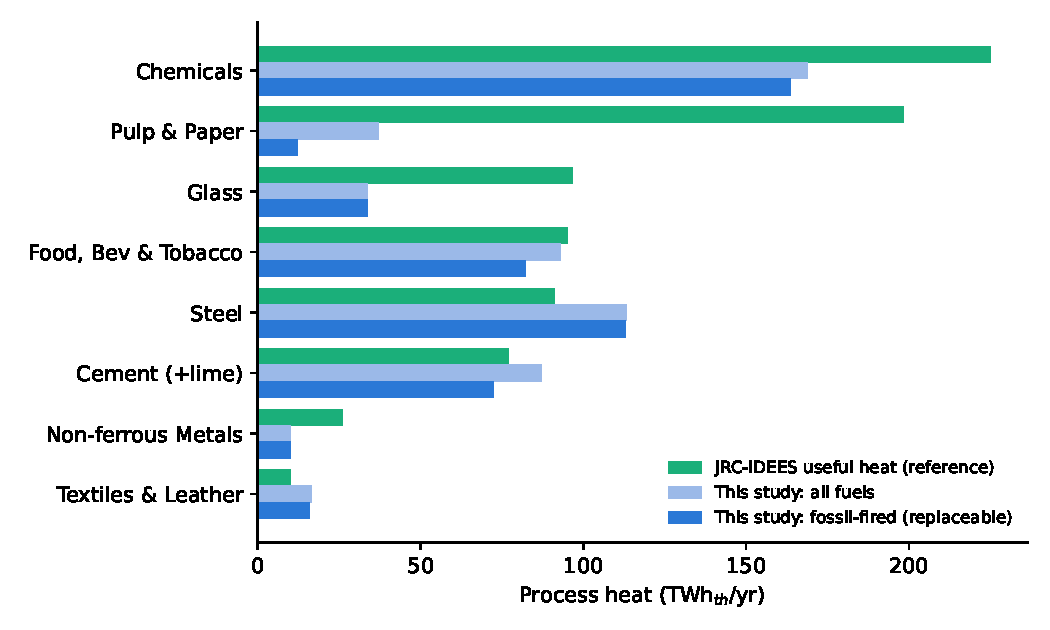
\includegraphics[width=0.85\textwidth]{figures/fig_heat_validation.pdf}
\caption{Validation of bottom-up process heat against JRC-IDEES useful heat for the EU-27, by sector. Bars show the JRC-IDEES reference (all fuels), this study's total heat from all fuels, and this study's fossil-fired (replaceable) heat.}
\label{fig:heatval}
\end{figure}

\subsection*{Supplementary Note 2: Estimation route and scope of replaceable heat}
Production is preferred to emissions where available because emissions are a less direct measure of process heat. Emissions include process emissions that do not come from fuel (for example, 60--65\% of cement CO$_2$ is from calcination), and they depend on the fuel mix, process design and system boundaries of each site, such as on-site electricity generation. Manz et al.\ compared production-based and emission-based estimates of fuel demand for individual sites and found that production data are more accurate, because process energy demand is more closely correlated with physical production than with emissions\cite{manz2018}. Emission-based estimates are therefore used only where production data are not available, which is the case for food and textiles. Fuel used as feedstock or reductant is excluded because it is incorporated into the product or consumed in a chemical reaction, so it cannot be replaced by an alternative heat source. Madeddu et al.\ likewise separate feedstock energy from electrifiable heat demand\cite{madeddu2020}. In steam cracking, byproduct methane and hydrogen recovered from the cracked gas supply most of the furnace fuel\cite{ren2006}. This fuel is fossil-derived, and an electrified furnace would have to supply the same duty, so it is included in the replaceable heat.

\subsection*{Supplementary Note 3: Temperature band assignment}
For facilities with production data, each sector or route is represented by one or more Hotmaps processes\cite{hotmaps2018}, weighted by tonnes of process per tonne of product (for example 1.2\,t sinter and 0.9\,t rolled steel per tonne of blast-furnace steel). The band shares are the mix of the processes' temperature distributions, weighted by each process's Hotmaps fuel SEC. Steel facilities that Climate TRACE lists under two routes (for example DRI-EAF and BF/BOF at the same site) use an equal 50/50 average of the two route recipes. Glass facilities are matched by name to a Hotmaps glass type (container, flat, fibre or other), and unmatched facilities use the EU production mix of 55\% container, 30\% flat, 5\% fibre and 10\% other glass. Alumina refineries have no Hotmaps process. Digestion and calcination use about 63--64\% and 31\% of refinery energy, with the remaining 5\% used by electric drives\cite{aac2023alumina,deloitte2022alumina}, so we assign 67\% of heat to digestion and 33\% to calcination. Digestion is heated by boiler steam supplied at 175--230\,$^\circ$C in low-temperature refineries and 325--400\,$^\circ$C in high-temperature refineries\cite{deloitte2022alumina}, and is assigned to the 200--500\,$^\circ$C band. Calcination takes place at about 1,100\,$^\circ$C\cite{barnes2024bayer} and is assigned to the $>$1000\,$^\circ$C band.

Food facilities are matched by name to a Hotmaps process (sugar, dairy, brewing, meat, bakery or starch). Food facilities with no name match, and all textile facilities, use the EU-27 useful heat of the food, beverages and tobacco sector, or of the textiles and leather sector, from the IndustryHeat-EU dataset\cite{industryheateu2025}, which applies the method of Madeddu et al.\cite{madeddu2020} to JRC-IDEES 2021 data. The dataset reports heat supplied directly to the process (for example by burners or hot water) by temperature range, and heat supplied as steam from boilers separately, without a temperature. We assume steam is supplied at 100--200\,$^\circ$C and assign direct heat at 100--400\,$^\circ$C to the 200--500\,$^\circ$C band. The resulting split is 20\% below 100\,$^\circ$C, 74\% at 100--200\,$^\circ$C and 6\% at 200--500\,$^\circ$C for food, and 32\% below 100\,$^\circ$C and 68\% at 100--200\,$^\circ$C for textiles, so all textile heat is served by heat pumps.

\begin{table}[h]
\centering
\small
\caption{Temperature band shares of process heat by sector and route (\% of heat). Shares are the SEC-weighted mix of the listed Hotmaps processes\cite{hotmaps2018}, with weights in tonnes of process per tonne of product. Assignment rules are described in Supplementary Note~3.}
\label{tab:bands}
\begin{tabular}{l p{0.36\textwidth} rrrrr}
\toprule
Sector & Route / processes (weight) & $<$100 & 100--200 & 200--500 & 500--1000 & $>$1000 \\
\midrule
Cement & Clinker calcination, dry (0.77) & 0 & 0 & 10 & 60 & 30 \\
Lime & Lime burning (1.0) & 0 & 0 & 0 & 40 & 60 \\
Glass & EU mix: container 0.55, flat 0.30, fibre 0.05, other 0.10 & 2 & 20 & 29 & 21 & 27 \\
 & Container or fibre glass (1.0) & 2 & 19 & 19 & 30 & 30 \\
 & Flat glass (1.0) & 2 & 21 & 43 & 12 & 22 \\
 & Other glass (1.0) & 2 & 22 & 22 & 22 & 32 \\
Iron and steel & BF/BOF: sinter 1.2, rolling 0.9 & 0 & 0 & 11 & 53 & 36 \\
 & EAF: EAF 1.0, rolling 0.9 & 0 & 0 & 0 & 17 & 83 \\
 & DRI-EAF: direct reduction 1.0, EAF 1.0, rolling 0.9 & 0 & 0 & 17 & 69 & 14 \\
 & BOF + EAF (equal mix) & 0 & 0 & 7 & 39 & 54 \\
 & DRI-EAF + BF/BOF (equal mix) & 0 & 0 & 15 & 66 & 19 \\
Steam cracking & Ethylene (1.0) & 0 & 0 & 0 & 100 & 0 \\
Chemicals & Ammonia (1.0) & 0 & 0 & 0 & 67 & 33 \\
 & Methanol (1.0) & 0 & 0 & 0 & 22 & 78 \\
 & Soda ash (1.0) & 30 & 40 & 0 & 0 & 30 \\
Aluminium & Primary smelting (1.0) & 0 & 0 & 0 & 100 & 0 \\
 & Alumina refinery: digestion 0.67, calcination 0.33\cite{aac2023alumina,deloitte2022alumina} (not Hotmaps) & 0 & 0 & 67 & 0 & 33 \\
Pulp and paper & Chemical pulp 0.5, paper 0.5 & 2 & 96 & 2 & 1 & 0 \\
 & Mechanical pulp 0.5, paper 0.5 & 5 & 88 & 5 & 2 & 0 \\
 & Unspecified: chemical pulp 0.35, mechanical pulp 0.15, paper 0.5 & 2 & 95 & 2 & 1 & 0 \\
Food & Unmatched: IndustryHeat-EU\cite{industryheateu2025} (not Hotmaps) & 20 & 74 & 6 & 0 & 0 \\
 & Dairy & 90 & 10 & 0 & 0 & 0 \\
 & Sugar & 10 & 60 & 0 & 30 & 0 \\
 & Brewing & 55 & 45 & 0 & 0 & 0 \\
 & Meat processing & 40 & 60 & 0 & 0 & 0 \\
 & Bread and bakery & 20 & 33 & 47 & 0 & 0 \\
 & Starch & 100 & 0 & 0 & 0 & 0 \\
Textiles & IndustryHeat-EU\cite{industryheateu2025} (not Hotmaps) & 32 & 68 & 0 & 0 & 0 \\
\bottomrule
\end{tabular}
\end{table}

\begin{table}[h]
\centering
\caption{Symbols used in the optimization model.}
\label{tab:symbols}
\begin{tabular}{>{$}l<{$} p{0.65\textwidth}}
\toprule
\textbf{Symbol} & \textbf{Meaning} \\
\midrule
k,\ K & Representative day and number of representative days (16) \\
t,\ H & Hour of the day and hours per day ($H = 24$, with $t-1 \equiv H$ when $t = 1$) \\
\mathcal{B}^{\HP},\ \mathcal{B}^{\IHB} & Bands served by heat pump (COP $>$ 1; $<$100 and 100--200\,$^\circ$C) or by IHB (COP $\leq$ 1; $\geq$200\,$^\circ$C) \\
g_{k,t} & Solar capacity factor in hour $t$ of representative day $k$ (MW per MW installed) \\
L_{b} & Flat heat load of band $b$ (MW$_{\mathrm{th}}$) \\
\sigma_{t} & Diurnal load shape, mean 1 (all 1 if flat) \\
y_{b,k,t} & IHB heat delivered to band $b$ \\
p_{j,k,t}^{\ch},\ p_{j,k,t}^{\dis},\ s_{j,k,t} & Charge, discharge and state of charge of storage $j$ \\
\eta_{j} & One-way efficiency of storage $j$, $\sqrt{\mathrm{RTE}_{j}}$ \\
h_{\max} & Maximum storage duration, 16\,h by default \\
AF & Availability factor, which sets the share of heat that must be served \\
P_{\PV}^{\max} & Optional solar cap from land limits (no cap if unset) \\
H & Number of hours in representative days \\
w_{k} & Weight of representative day $k$ (number of days it represents) \\
x_{b,k,t}^{\mathrm{dir}},\ x_{b,k,t}^{\mathrm{batt}} & Electricity to the heat pump of band $b$ directly from solar or from the Li-ion battery \\
u_{b,k,t} & Unserved heat in band $b$ \\
\mathrm{COP}_{b} & Heat pump coefficient of performance for band $b$ \\
P_{b}^{\HP},\ P_{j}^{\ch},\ P_{j}^{\dis},\ E_{j} & Heat pump capacity, storage charge and discharge power, and storage energy capacity \\
c_{\PV},\ c_{\Li,E},\ c_{\Li,P},\ c_{\IHB,\cdot},\ c_{b}^{\HP} & Annualised unit costs of each technology \\
\mathrm{RTE}_{j} & Round-trip efficiency of storage $j$ (0.90 Li-ion, 0.95 IHB) \\
x & Electricity \\
\bottomrule
\end{tabular}
\end{table}

\end{document}